\section{Innledning}

%I innledningen skal du plassere deg i fagfeltet og vise at du har kjennskap til tidligere forskning. Innledningen skal gjøre rede for hva vi vet og hva vi ikke vet om feltet.

%Dette gjør du ved å presentere:

%et problem eller et fenomen du skal studere

\begin{figure} 
\begin{center} 
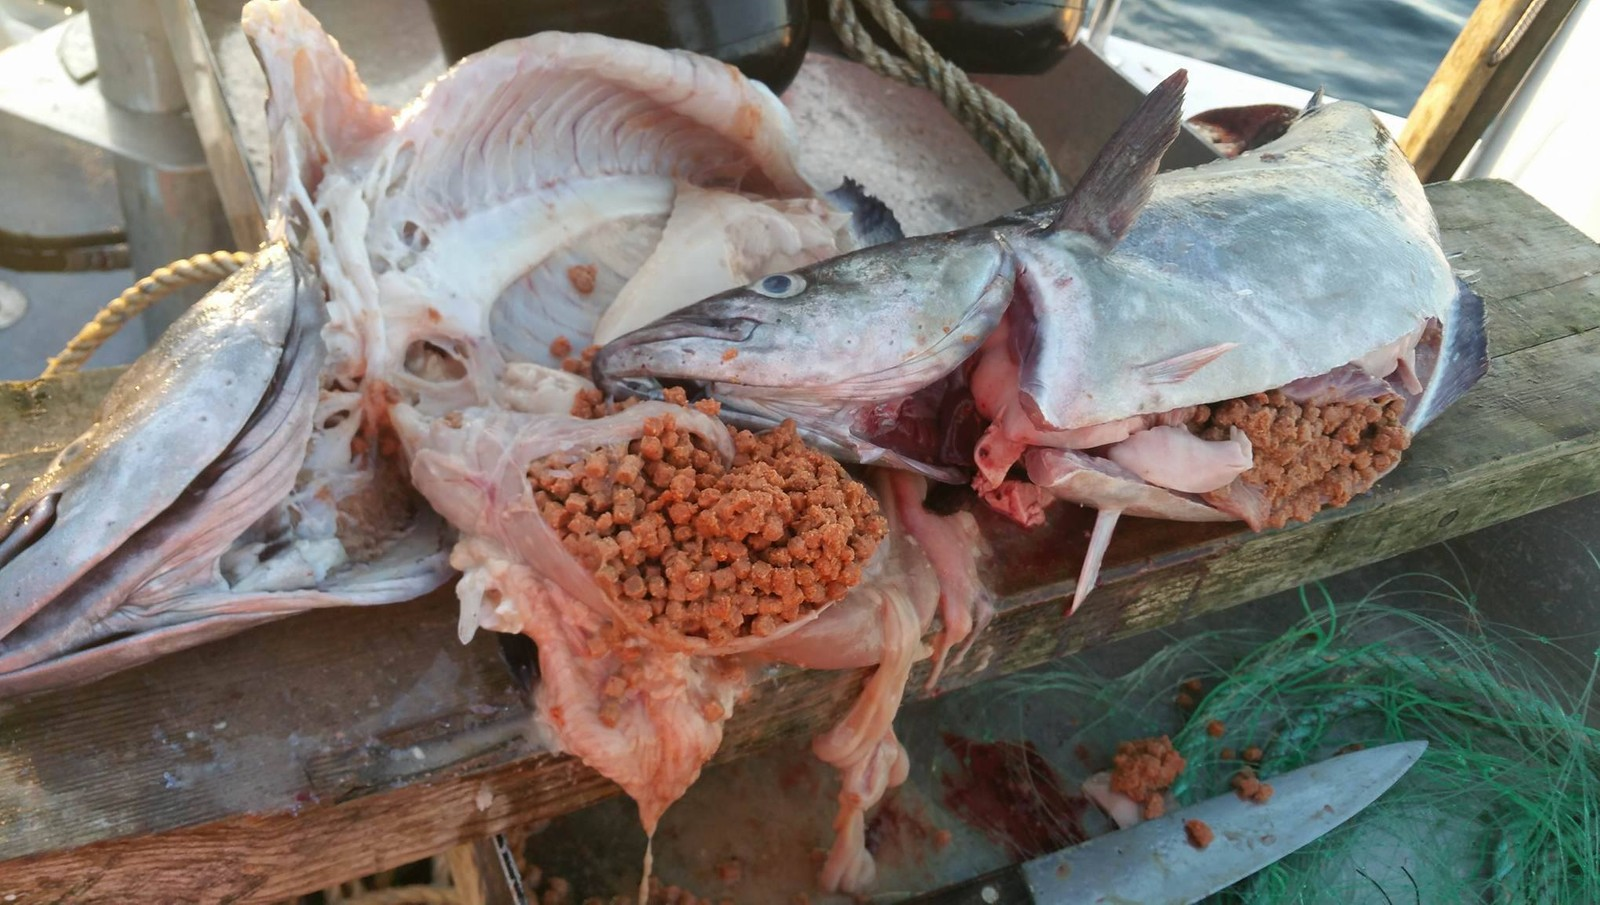
\includegraphics[scale=0.2]{figures/oppdrettfor}
\caption{\small \sl Figuren viser et eksempel av ``pellets-fisken''. Det lukter ekkelt og det er forferdelig å sløye en fôrsprengt fisk, ifølge flere fiskere som har vært i kontakt med NRK \cite{Trana m.fl. 2019}. Seien har vært under merdene, da blir den full av pellets. Fôrsprengt fisk er unaturlig, hode blir for liten og kroppen for stor. Dette har pågått i mange år. Likevel blir fisken omsatt, fiskere får levert slik fisk til enkelte fiskebruk. \cite{Angell og Ekanger 2017} \label{fig:oppdrettfor}} 
\end{center} 
\end{figure} 

\begin{figure}
\begin{center} 
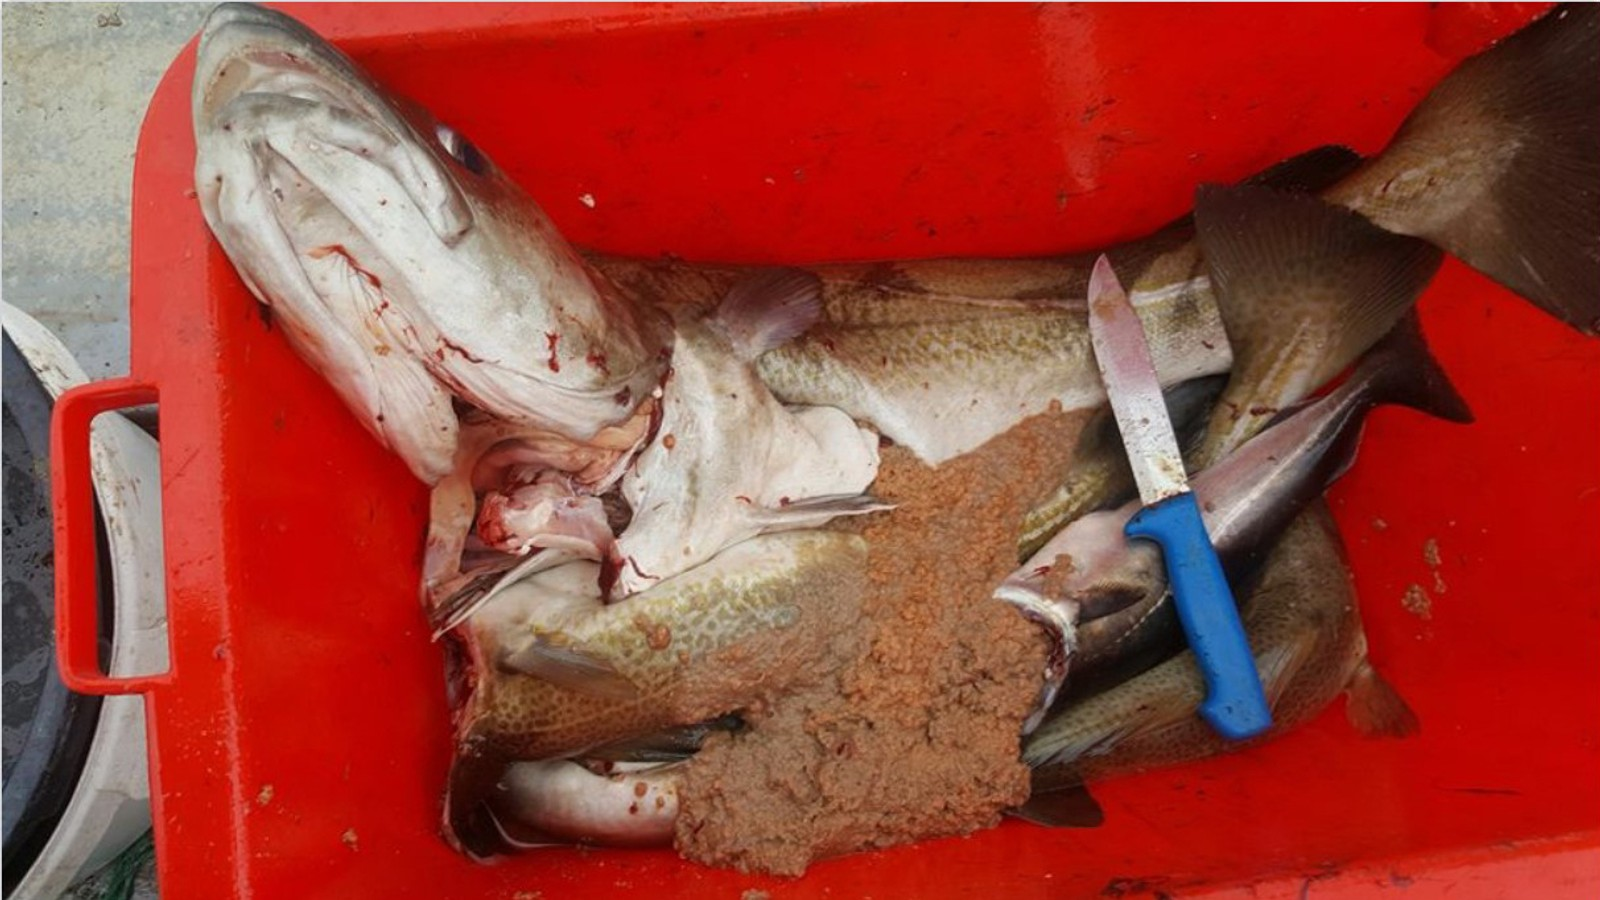
\includegraphics[scale=0.2]{figures/forsprengt}
\caption{\small \sl Figuren viser et eksempel av fôrsprengt fisk. Det lukter ekkelt og det er forferdelig å sløye en fôrsprengt fisk, ifølge flere fiskere som har vært i kontakt med NRK. Foto: Arnold Jensen. \cite{Trana m.fl. 2019} \label{fig:forsprengt}} 
\end{center} 
\end{figure} 

Kystfiskere hevder villfisken får i seg så mye laksefôr at fiskeplassene blir ødelagt. ``Litt overraskende utspill'' svarer oppdrettsbransjen. Fisker Tor Inge Larsen i Brønnøysund sa til NRK i 2018 at han fortviler over det han mener er dårligere kvalitet hos fisken han fanger. Han sa han kan knapt huske sist han fikk en sei om bord i båten uten at den hadde pellets fra lakseoppdrett i magen. Han hevder fiskerne har blitt frastjålet fiskeområder på høylys dag, og mener fiskefeltene nært Brønnøysund på Sør-Helgeland i Nordland har fått betydelig lavere kvalitet på grunn av oppdrettsanleggene. \cite{Olsen m.fl. 2018}

Johnny Eliassen som er bosatt på Reinøya i Troms, Karlsøy kommune, fortalte til NRK at han hadde tidligere engasjert seg i saken for å hindre at kystområdet ble lokasjon for oppdrettsanlegg. Det ble allikevel åpnet et oppdrettsanlegg mai 2017 i fjorden på Reinøya, og det hevder de lokale fiskerne at de har merket. De har fisket ``pelletstorsk'',  torsk med magen full av pellets, selv over en kilometer unna anlegget. Oppdrettere reklamerer oppdrettsfisk som den absolutte beste fisken. Eliassen kunne ikke tenke seg er at det virkelig er tilfelle, for lukten og konsistensen på fisken gjør den uspiselig i hans øyne. \cite{Jakobsen 2017}

Men fiskerne og forskerne har vært uenige om hvorvidt pellets fra lakseoppdrett påvirker kvaliteten av vill fisk som spiser den. Det er forsket relativt lite på hvordan oppdrett påvirker villfisk. Seniorrådgiver Bjørn-Steinar Sæther fra Nofima ga ut en artikkel i 2017 der han mener seien som hadde spist oppdrettsfôr får en litt bløtere og noe mer spaltet muskel enn annen sei, men den var fortsatt stort sett innenfor kategorien god kvalitet. \cite{Saether 2017}

Kommunikasjonsdirektør Are Kvistad i Sjømat Norge er litt overrasket over utspillet fra fiskeren på Helgeland. Han mener laksepellets ikke utgjør noen fare for villfisk. ``Det er et fiskefôr som blir sjekket av myndighetene, og er et trygt og næringsrikt fôr som også er trygt for villfisk'', sa Kvistad til NRK i 2018. Kvistad mente det også er i oppdretternes interesse, både økonomisk og utslippsmessig, å redusere fôringen av oppdrettslaksen slik at den kun får den maten den trenger. \cite{Olsen m.fl. 2018}

Vinteren 2018 rømte 52 000 laks fra Marine Harvests oppdrettsanlegg i Nærøy kommune i Trøndelag. Ifølge Namdalsavisa inneholdt laksen medisiner mot innvollsorm. Mattilsynet gikk ut og sa at det var trygt å spise fisken, men at den ikke kunne omsettes videre. \cite{nrk 2018}

Den rømte laksen hadde blitt gitt medisinfôr med praziquantel og skulle være i karantene i 14 dager. For fiskere, slik som Arnold Jensen, som har snakket med naturvernforbundet, er denne informasjonen skremmende. Han ønsker at mattryggheten til villfisk som beiter ved oppdrettsanleggene skal kontrolleres. Se figur \ref{fig:oppdrettfor} og \ref{fig:forsprengt}. \cite{Christensen 2019}

I 2019 kom ``pellets-fisken'' i medienes søkelys igjen, denne gangen var det fiskere i Lyngen kommune i Troms som slo alarm. Villfisk som hadde spist oppdrettsfôr som inneholdt medisin omsettes av fiskere i fjorden. De ønsker svar på om det kan være farlig for forbrukere. \cite{Trana m.fl. 2019}

\begin{figure} 
\begin{center} 
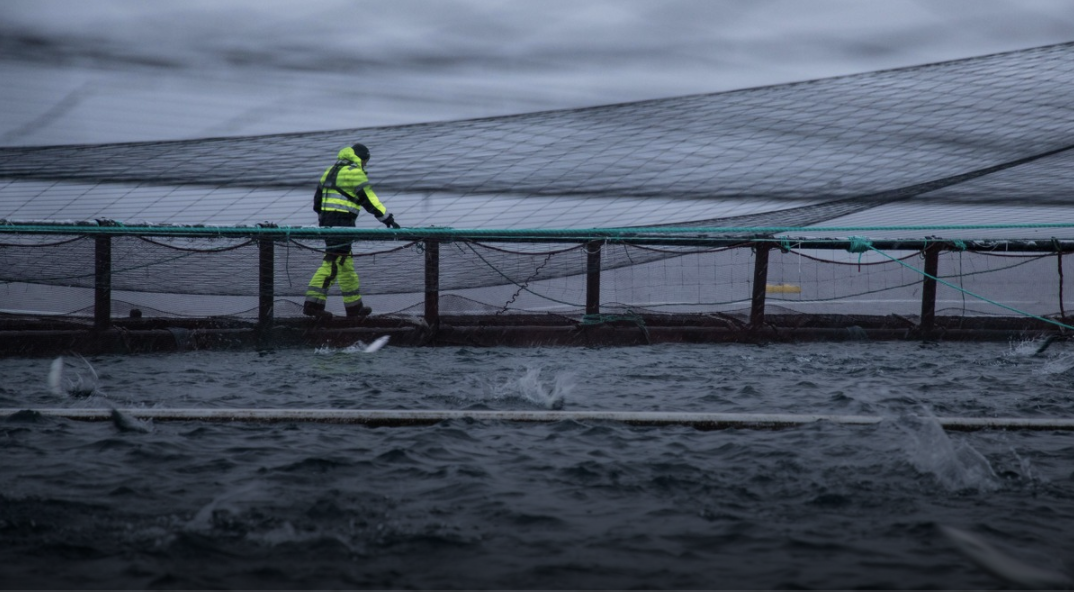
\includegraphics[scale=0.7]{figures/oppdrett}
\caption{\small \sl Figuren viser et oppdrettsanlegg. \cite{Olsen m.fl. 2018} \label{fig:anlegg}} 
\end{center} 
\end{figure} 

%bakgrunnen for valg av tema
%problemstillingen eller hypotesene du skal undersøke
%På slutten av introduksjonen kan du også si noe om hvordan du har tenkt å strukturere resten av oppgaven, som en kort leserguide.

%Et tips er å begynne å skrive på innledningen tidlig, slik at den kan gi retning for det videre arbeidet ditt. Så går du heller over innledningen igjen på slutten for å skrive den helt ferdig. Da får du en innledning som har god sammenheng med resten av teksten.

Sjømatdivisjonen og Akvadivisjonen ved Nofima har en strategisk internsatsing som går ut på å samle kunnskap om sameksistens mellom ulike marine næringer og interesser, deriblant om hvordan man kan unngå konflikter mellom ulike interesser. \cite{Robertsen 2020}

En av problemstillingene er sameksistens mellom fiskeri- og oppdrettsnæringene, og hvordan oppdrettsanlegg påvirker de nærliggende fiskeplassene. I den forbindelse er det interessant å kartlegge omfanget av hvitfisk som beiter på fôr fra oppdrettsanlegg. Dette er en problemstilling som har vært i fokus hos media etter at flere fiskere har fanget fôrsprengt torsk og sei i fjorder hvor det finnes oppdrettsanlegg. Det hevdes at denne fisken er av betydelig dårligere kvalitet og den kan ha fått i seg medisiner gjennom fôret som gjør at den kan være farlig å spise. \cite{Olsen 2019}

Det behøves kunnskap om hvor mange villfisk som trekker til oppdrettsanlegg, og under hvilke forhold, slik at man kan komme nærmere en løsning som kan dempe konflikten mellom disse to næringene. 

Målet med dette prosjektet var å utvikle et system som kan telle antall villfisk av ulike arter basert på en videostrøm fra et undervannskamera. Det er ønskelig å kunne vise resultatet som en fordeling av observasjoner over tid for hver art. 

\subsection{Delmål}

\subsubsection{Programvare skrevet i C++}

Prosjektet består i hovedsak av å utvikle en programvare som kan gjøre følgende ved hjelp av maskinlæring: 

\begin{enumerate}
\item Segmentere fisk fra bakgrunn
\item Klassifisere hver fisk etter art
\item Spore hver fisk gjennom hvert bilde i videostrømmen inntil fisken forlater kameraets synsfelt
\end{enumerate}

Programvaren implementeres i C++ ved hjelp av OpenCV-biblioteket\footnote{https://opencv.org/}. Det kan også være aktuelt å lage et grafisk grensesnitt hvor tellingene fra hver art kan vises i sanntid, men dette er avhengig av om prosjektets omfang tillater det. 